\documentclass[10pt,letterpaper]{article}

% Not sure what this does:
\usepackage[top=0.85in,left=2.75in,footskip=0.75in]{geometry}

% amsmath and amssymb packages, useful for mathematical formulas and symbols
\usepackage{amsmath,amssymb,bm}

% Use adjustwidth environment to exceed column width (see example table in text)
\usepackage{changepage}

% Use Unicode characters when possible
\usepackage[utf8x]{inputenc}

% textcomp package and marvosym package for additional characters
\usepackage{textcomp,marvosym}

% cite package, to clean up citations in the main text. Do not remove.
\usepackage{cite}

% Use nameref to cite supporting information files (see Supporting Information section for more info)
\usepackage{nameref}
\usepackage[colorlinks = true, urlcolor = blue]{hyperref}

% line numbers
\usepackage[right]{lineno}

% ligatures disabled
\usepackage{microtype}
\DisableLigatures[f]{encoding = *, family = * }

% color can be used to apply background shading to table cells only
\usepackage[table]{xcolor}

% array package and thick rules for tables
\usepackage{array}

% create "+" rule type for thick vertical lines
\newcolumntype{+}{!{\vrule width 2pt}}

% create \thickcline for thick horizontal lines of variable length
\newlength\savedwidth
\newcommand\thickcline[1]{%
  \noalign{\global\savedwidth\arrayrulewidth\global\arrayrulewidth 2pt}%
  \cline{#1}%
  \noalign{\vskip\arrayrulewidth}%
  \noalign{\global\arrayrulewidth\savedwidth}%
}

% \thickhline command for thick horizontal lines that span the table
\newcommand\thickhline{\noalign{\global\savedwidth\arrayrulewidth\global\arrayrulewidth 2pt}%
\hline
\noalign{\global\arrayrulewidth\savedwidth}}


% Remove comment for double spacing
%\usepackage{setspace} 
%\doublespacing

% Text layout
\raggedright
\setlength{\parindent}{0.5cm}
\textwidth 5.25in 
\textheight 8.75in

% Bold the 'Figure #' in the caption and separate it from the title/caption with a period
% Captions will be left justified
\usepackage[aboveskip=1pt,labelfont=bf,labelsep=period,justification=raggedright,singlelinecheck=off]{caption}
\renewcommand{\figurename}{Fig}

% Use the PLoS provided BiBTeX style
\bibliographystyle{plos2015}

% Remove brackets from numbering in List of References
\makeatletter
\renewcommand{\@biblabel}[1]{\quad#1.}
\makeatother

% Leave date blank
\date{}

% Header and Footer with logo
\usepackage{lastpage,fancyhdr,graphicx}
\usepackage{epstopdf}
\pagestyle{myheadings}
\pagestyle{fancy}
\fancyhf{}
\setlength{\headheight}{27.023pt}
%\lhead{\includegraphics[width=2.0in]{PLOS-submission.eps}}
\rfoot{\thepage/\pageref{LastPage}}
\renewcommand{\footrule}{\hrule height 2pt \vspace{2mm}}
\fancyheadoffset[L]{2.25in}
\fancyfootoffset[L]{2.25in}
\lfoot{\sf PLOS}

%% Include all macros below

\newcommand{\lorem}{{\bf LOREM}}
\newcommand{\ipsum}{{\bf IPSUM}}

%% Customized Macros
\usepackage{booktabs}
\usepackage{multirow}

%% For inline code
\usepackage{listings,lstautogobble}
\newcommand{\inlinecode}[1]{\lstinline{#1}}
% Custom Python Syntax
\lstset
{
    basicstyle=\small\ttfamily,
    frame=L,
    morekeywords={True, False},
    numbers=left,
    numbersep=10pt,
    showstringspaces=false,
    tabsize=3,
}
  
  %%%%%%%%%%%%%%%%%%%%%%%%%%
  
% Some new commands specific to RNA Stat paper

%\newcommand{\its}{{\it single}}
%\newcommand{\itd}{{\it double}}
%\newcommand{\itt}{{\it transitional}}


\begin{document}
\vspace*{0.2in}


\begin{flushleft}
{\Large
\textbf\newline{Base-pair Ambiguity and the Kinetics of RNA Folding} 
}
\newline
\\
Guangyao Zhou\textsuperscript{1*},
Jackson Loper\textsuperscript{2},
Matthew T. Harrison\textsuperscript{1},
Stuart Geman\textsuperscript{1}
\\
\bigskip
\textbf{1} Division of Applied Mathematics, Brown University, Providence, RI, USA
\\
\textbf{2} Data Science Institute, Columbia University, New York, NY, USA
\\
\bigskip

* guangyao\_zhou@brown.edu

\end{flushleft}

% Please keep the abstract below 300 words
%\section*{Abstract}
%NEEDS TO BE EDITED...!!!
%Non-coding RNA molecules contribute to cellular function through diverse roles, including genome regulation, DNA and RNA repair, RNA splicing, catalysis, protein synthesis, and intracellular transportation  \cite{Morris2014-iu,Kung2013-se}. The mechanisms of these actions can only be fully understood in terms of native secondary and tertiary structures. When provided with a sufficient number of homologous sequences, the gold standard for secondary structure prediction continues to be comparative analysis  \cite{Gutell1992-hu}. Alternatively, the prevailing {\em computational} approach to secondary structure is through the Gibbs (thermal) equilibrium, by Monte Carlo sampling or approximating the minimum free energy (MFE) configuration \cite{Mathews1999-hc,Zuker1999-rc}. Aside from the necessary approximations, an enduring debate concerns the biological relevance of equilibrium configurations \cite{Levinthal1969-hi,Higgs2000-gj,Flamm2008-ir, Baker1994-px}. Here we adopt a kinetic perspective and argue that the existence of reliable folding on biologically relevant time scales suggests an {\em intra-molecular} statistical relationship between secondary and {\em primary} structures: as compared with other locations, nucleotide sequences in and around secondary-structure stems will have fewer Watson-Crick and wobble matches that are inconsistent with the native structure. An ``ambiguity index'', one for each pair of molecule and presumed secondary structure, measures the prevalence of false matches and hence the tendency to form metastable structures  incompatible with native structures. The ambiguity index statistically separates an ensemble of RNA molecules that operate as single entities (Group I and II Introns) from an ensemble that operates as protein-RNA complexes (SRP and tmRNAs), and ensembles of secondary structures determined by comparative analysis from ones based on thermal equilibrium. We find lower average ambiguity in single-entity RNA's than protein-RNA complexes, and, among single-entity RNA's, lower ambiguity with comparative analyses than equilibrium analyses. Both comparisons are supported by exact and highly significant hypothesis tests. These experiments, motivated by a hypothesized mechanism of folding, and the first of their kind, are consistent with folding to metastable but not necessarily equilibrium structures. 
%
%
%% Please keep the Author Summary between 150 and 200 words
%% Use first person. PLOS ONE authors please skip this step. 
%% Author Summary not valid for PLOS ONE submissions.   
%\section*{Author Summary}
%Recent discoveries indicate that, in addition to being a messenger between DNA and protein, RNA molecules assume a wide range of biological functions. For biological macromolecules, structure is function. Experimental determination of RNA structures is still time-consuming, and computational approaches are of great importance. The prevailing computational approach tries to find the structure with the minimum energy, yet the relevance of this minimum energy structure to the native structure is still hotly debated. In this paper, we adopt a kinetic perspective, and argue that more emphasis should be placed on the folding process when trying to develop computational methods for RNA structure prediction. We present some statistical analyses using the primary and secondary data (sequence and base-pairs data) of RNA molecules, based on the concept of ``local ambiguity", i.e. the molecule's tendency to ``make a mistake" at a certain location when forming secondary structures. Our results highlight deficiencies in the minimum-energy approach, and demonstrate the importance of considering kinetics as well as protein-RNA interactions in developing computational approaches for RNA secondary structure prediction.

\linenumbers

% Use "Eq" instead of "Equation" for equation citations.
\section*{Introduction}

Discoveries in recent decades have established a wide range of biological roles served by RNA molecules, in addition to their better-known role as carriers of the coded messages that direct ribosomes to construct specific proteins. Non-coding RNA molecules participate in gene regulation, DNA and RNA repair, splicing and self-splicing, catalysis, protein synthesis, and intracellular transportation \cite{Morris2014-iu,Kung2013-se}. To understand the mechanisms of these actions, emphasis has to be placed on the native structures, both secondary and tertiary. Our focus here will be on secondary structure, often a vital intermediary, and a useful abstraction for understanding the functions of non-coding RNA molecules \cite{Higgs2000-gj}.

Because of the time-consuming nature of experimental determination of RNA structures, a considerable amount of work has been put into computational (as opposed to experimental) approaches. For secondary structure prediction, comparative analysis is the gold standard  \cite{Gutell1992-hu}. But accurate comparative analysis typically requires a large number of homologous sequences, which may or may not be available. On the other hand, the prevailing {\em computational} approaches  XXX References??? XXX are based on an important and controversial assumption. Namely, that the structures of  non-coding RNA molecules, {\em in vivo}, are in thermal equilibrium. If this were the case, and if the configuration energies could be accurately specified, then secondary (and in principle, even tertiary) structures could be explored through Monte Carlo sampling of the Gibbs equilibrium distribution. (XXX or is it the Boltzmann equilibrium??? XXX) Alternatively, depending on the nature of the energy landscape, secondary structures could be approximated by identifying the minimum free energy (MFE) configuration  \cite{Mathews1999-hc,Zuker1999-rc}. However, even if we put aside the necessity for approximations, the biological relevance of equilibrium configurations has been a source of misgivings at least since 1969, when Levinthal pointed out that the time required to equilibrate might be too long by many orders of magnitude  \cite{Levinthal1969-hi}. In light of these observations, and considering the ``frustrated'' nature of the folding landscape, many have argued that when it comes to structure prediction for macromolecules, kinetic accessibility is more relevant than equilibrium thermodynamics  \cite{Higgs2000-gj,Flamm2008-ir,Baker1994-px}.

The primary structures of RNA molecules typically afford many opportunities to form short or medium-length stems\footnote{
By which we will mean sequences of G$\cdot$U (``wobble pairs'') and/or Watson-Crick pairs.},
most of which do not participate in the native structure. This situation not only makes it hard for the biologist to accurately predict secondary structure, but equally challenges the molecule to avoid these ``energetic traps.'' Once formed, they require a large amount of energy (not to mention time) to be unformed. By what mechanisms might these traps be discouraged, if not actually avoided? 
Ideally, the only stems available in the primary structure would be those that participate in the secondary structure, but this is obviously too restrictive for all but the shortest or simplest of the structural RNA molecules. Still, there can be little doubt that the necessity for repeatable and efficient folding produces a selective pressure against the more disruptive ambiguities---e.g.
a sequence that can form half of either of two stems, both of which are kinetically accessible and stable, but only one of which is native, or a sequence that is unpaired in the native structure but can nonetheless form a stem that is stereochemically inconsistent with the native structure. By this reasoning, which emphasizes kinetics rather than equilibrium, {\em per se}, we might expect to find information in the intra-molecular ambiguities about the folding process, or even the native structure.  

We will introduce quantitative measures of ambiguity and demonstrate their statistical relationships to native secondary structure and to qualitative distinctions between RNA families.
Using a somewhat arbitrary convention, we will
refer to sequences of length four (four consecutive nucleotides) as {\em segments}. Keeping this convention in mind, each line of statistical
evidence is based on the same formal definition of the ``local ambiguity'' of a given segment. This is simply the number of its complementary pairs in the molecule. 
When we refer to the {\em location} of a segment, we will mean the location of the first element of the segment, counting from 5$^\prime$ to 3$^\prime$, and  
when we refer to the local ambiguity of a location, we will mean the local ambiguity of the segment at that location. 
Local ambiguity is an intrinsic property of the primary structure. We will be interested in exposing its statistical relationships to any given candidate secondary structure of the same molecule. For this purpose, for any particular secondary structure we distinguish three different kinds of locations:
\begin{description}
	\item[\textit{Single}:] Locations where all nucleotides in the corresponding segment are unpaired in the secondary structure;
	\item[\textit{Double}:] Locations where all nucleotides in the corresponding segment are paired in the secondary structure;
	\item[\textit{Transitional}:] Locations where some nucleotides in the corresponding segment are paired and others are unpaired in the secondary structure.
\end{description}
{\em Double} and {\em transitional} locations participate in the candidate secondary structure, while {\em single} locations do not.
As a general rule, local ambiguities measured at any of these locations will increase with the length of the molecule---there are simply more opportunities to find complementary sequences.
Instead of using the local ambiguities themselves, we focus on the {\em differences} between ambiguities in and around stems ({\em double} and {\em transitional} locations) from those at unpaired ({\em single}) locations. In particular, we defined the ``T-S ambiguity index'' to be the difference between the average local ambiguity at {\em transitional} locations minus the average at {\em single} locations. We defined the ``D-S ambiguity index'' similarly, but adjusted for the evident bias at {\em double} locations, each of which, after all, has at least one complementary pair somewhere in the molecule. The D-S ambiguity index, then, is the average local ambiguity at {\em double} locations minus the average over those {\em single} locations that have at least one ambiguity.

Using only primary and (comparative-analysis) secondary structures, elementary counting statistics, 
and exact, distribution-free, tests,
we will give evidence that
both the T-S and D-S ambiguity indexes 
significantly separate two groups of non-coding RNA molecules: one group consists of  RNA families that operate, {\em in vivo}, as single entities---the Group I and Group II Introns;
the other group is made up of RNA families  known to be active as protein-RNA complexes (i.e. as ribonculeoproteins)---the transfer-messenger RNAs (tmRNA), the RNAs of signal recognition particles (SRP RNA), the ribonuclease P family (RNase P), and the 16s and 23s ribosomal RNAs (16s and 23s rRNA). In particular, ``unbound'' RNA molecules, which perform their functions without being part of a larger nucleoprotein complex, have systematically lower T-S and D-S ambiguity indexes than the ``bound'' RNA molecules found in ribonucleoproteins. 
There are many possible explanations---see {\em Discussion}. Possibly, the unbound molecules are more sensitive to ambiguities and their energy traps, especially those ambiguities that involve the structurally critical {\em double} and {\em transitional} regions, then the bound molecules, whose secondary structures may well be influenced by their chemical relationships to proteins. Interestingly, this distinction between the ambiguity indexes of bound and unbound molecules largely disappears when MFE structures are used instead of comparative-analysis structures in defining {\em double}, {\em transitional}, and {\em single} locations. In fact, for most unbound molecules we can classify a candidate secondary
structure (was it derived from comparative analysis or by a minimum-free-energy calculation?) just by looking at the difference in the T-S or the D-S index under the two structures.

The {\em Results} section is organized as follows:  we first develop some basic notation and definitions, and then present an exploratory and largely informal statistical analysis. This is followed by formal results comparing ambiguities in unbound versus bound molecules, and then by a comparison of the ambiguities implied by secondary structures derived from comparative analyses to those derived through minimization of free energy. 
The {\em Results} section is followed by a {\em Discussion}, and then by the section on {\em Materials and Methods}, which, among other things, includes detailed information about the data and its (open) source, as well as links to code that can be used to reproduce our results or for further experimentation. 

\section*{Results}

\subsection*{Basic Notation and Definitions}

Consider a non-coding RNA molecule with $N$ nucleotides.  Counting from 5$^\prime$ to 3$^\prime$, we denote the primary structure by
\begin{equation}
p = (p_1, p_2, \cdots, p_N)  , \text{where }p_i \in \{ A, G, C, U \}, i = 1, \cdots, N
\end{equation}
and the secondary structure by
\begin{equation}
s = \left\{ (j, k) :\text{nucleotides $j$ and $k$ are paired, $1 \leq j < k \leq N$} \right\}
\end{equation}
and we define the {\em segment} at {\em location} $i$ to be 
\begin{equation}
	P_i = (P_{i, 1}, P_{i, 2},P_{i, 3}, P_{i, 4}) = (p_i, p_{i + 1},p_{i + 2},p_{i + 3})
\end{equation}
There is no particular reason for using segments of length four, and in fact all qualitative conclusions are identical with segment lengths three, four, or five, 
and, for that matter, whether or not we include the G$\cdot$U wobble pairs. 
We chose to include them.

Which segments are viable complementary pairs to $P_i$? The only constraint on location is that an RNA molecule cannot form a loop of two or fewer nucleotides. Let $A_i$ be the set of all segments that are potential pairs of $P_i$:
\begin{equation}
A_i = \{P_j: 1 \leq j \leq i - 7 \text{ or }i + 7 \leq j \leq N - 3\}
\end{equation}
We can now define the {\em local ambiguity function}, 
\[
a(p) = (a_1(p), \cdots, a_{N - 3}(p))
\]
which is a vector-valued function of the primary structure $p$. The vector has  one component, $a_i(p)$, for each segment $P_i$, which is, simply, the number of feasible segments that are complementary to $P_i$:
\begin{align}
 a_i (p)& =  \# \{ P \in A_i : P \text{ and }P_i \text{ are complementary} \}  
 \\
& = 
\#\big\{P_j\in A_i:  (P_{i, k}, P_{j, 5 - k}) \in \{ (A, U), (U, A), (G, C), (C, G), (G,U), (U,G) \},
\nonumber \\
&  \ \ \ \ \ \ \ \ k=1,\ldots,4 \big\} 
\nonumber 
\end{align}

We want to explore the relationship between ambiguity and secondary structure. 
We can do this conveniently, on a molecule-by-molecule basis, by introducing another vector-valued function, this time depending only on a purported secondary structure.  Specifically, the new function assigns a descriptive label to each location (i.e. each nucleotide), determined by whether the segment at the given location is fully paired, partially paired, or fully unpaired. 

Formally, given a secondary structure $s$, as defined in equation (2), and a location $i\in\{1, 2,\ldots,N-3\}$, let $f_i(s)$ be the number of nucleotides in $P_i$ that are paired under $s$:
\begin{equation}
f_i(s) = \#\{j\in P_i:(j,k)\in s\text{ or } (k,j)\in s, \text{ for some } 1\leq k \leq N\}
\end{equation}
Evidently, $0\leq f_i(s)\leq 4$. The ``paired nucleotides function'' is then the 
vector-valued function of secondary structure defined as 
$f(s)=(f_1(s),\ldots,f_{N-3}(s))$.
Finally, we use $f$ to distinguish three types of locations (and hence three types of segments): location $i$ will be labeled 
\begin{equation}
	\begin{cases}
		\text{\textit{single} if } f_i(s) = 0 \\
		\text{\textit{double} if } f_i(s) = 4 \\
		\text{\textit{transitional} if } 0 < f_i(s) < 4
	\end{cases} i = 1, 2, \cdots, N - 3
\end{equation}

\subsection*{A First Look at the Data: Shuffling Nucleotides}
Our goal is to explore connections between ambiguities and basic characteristics of RNA families, as well as the changes in these relationships, if any, when using comparative, as opposed to MFE, secondary structures.
For each molecule and each location $i$, the segment at $i$ has been assigned a ``local ambiguity'' $a_i(p)$ that depends only on the primary structure, and a label ({\it single}, {\it double}, or {\it transitional}) that depends only on the secondary structure. Since the local ambiguity, by itself, is strongly dependent on the length of the molecule, and possibly on other intrinsic properties,
we proposed two {\em relative} ambiguity indexes: T-S and D-S, each of which depends on both the primary ($p$) and purported secondary ($s$) structures. Formally,
\begin{equation}
	d_\text{T-S}(p, s) = \frac
	{\sum_{j = 0}^{N - 3} a_j (p) 
	c^{\text{tran}}_j (s)}
	{\sum_{j = 0}^{N - 3} 
	c^{\text{tran}}_j (s)} - 
	\frac
	{\sum_{j = 0}^{N - 3} a_j (p) c_j^{\text{single}} (s)}
	{\sum_{j = 0}^{N - 3} c_j^{\text{single}} (s)}
\end{equation}
where we have used
$c_i^{\text{double}}$ and $c_i^{\text{single}}$ for indicating whether location $i$ is {\it transitional} or {\it single} respectively. In other words, for each $i=1,2,\ldots,N-3$
\begin{align}
	c_i^{\text{tran}} &=
	\begin{cases}
		1, & \text{if location $i$ is \textit{transitional}} \\
		0, & \text{otherwise}
	\end{cases} \\
	c_i^{\text{single}} &=
	\begin{cases}
		1, & \text{if location $i$ is \textit{single}} \\
		0, & \text{otherwise}
	\end{cases}
\end{align}
In short, the T-S ambiguity index is the difference in the averages of the local ambiguities at {\em transitional} sites and {\em single} sites.
Since, as noted earlier, the local ambiguity at every {\em double} location, $i$, is at least one ($a_i\geq 1$), the D-S index involves only those {\em single} locations, $j$, for which it is also the case that $a_j\geq 1$:
\begin{equation}
	d_\text{D-S}(p, s) = \frac
	{\sum_{j = 0}^{N - 3} a_j (p) 
	c^{\text{double}}_j (s)}
	{\sum_{j = 0}^{N - 3} 
	c^{\text{double}}_j (s)} - 
	\frac
	{\sum_{j = 0}^{N - 3} a_j (p) \hat{c}_j^{\text{single}} (p,s)}
	{\sum_{j = 0}^{N - 3} \hat{c}_j^{\text{single}} (p,s)}
\end{equation}
Here, $\hat{c}^{\text{single}}$, which evidently depends on both primary and secondary structure, indicates those {\em single} locations with at least one pair: for each $i=1,2,\ldots,N-3$
\begin{align}
	\hat{c}_i^{\text{single}} & =
	\begin{cases}
		1, & \text{if location $i$ is \textit{single} and $a_i(p)\geq 1$} \\
		0, & \text{otherwise}
	\end{cases}
\end{align}

Thinking kinetically, we might expect to find relatively small values of the T-S and D-S indexes
($d_\text{T-S}$ and $d_\text{D-S}$)
in RNA families which fold and operate as individual entities---what we call here the unbound RNA. One reason for believing this
is that larger numbers of partial matches for a given sequence in or around a stem would likely interfere with the {\em nucleation} of the native stem structure, potentially disrupting folding, and nucleation appears to be a critical and perhaps even rate-limiting step in folding. 
Indeed, the experimental literature  \cite{Porschke1974-hn, Porschke1974-nr, Porschke1977-xz, Mohan2009-gt} has long suggested that stem formation in RNA molecules is a two-step process. When forming a stem, there is usually a slow nucleation step, resulting in a few consecutive base pairs at a nucleation point, followed by a fast zipping step. 
Since the ambiguity indexes are functions of the secondary structure, $s$, 
our expectation are made, implicitly, under the assumption that $s$ is correct. For the time being we will focus only on comparative structures, returning later to the questions about MFE structures raised in the {\em Introduction}. 

How are
we to gauge $d_\text{T-S}$ and $d_\text{D-S}$, and how are we to compare their values across different RNA families? 
Consider the following experiment: for a given RNA molecule we create a ``surrogate'' which has the same nucleotides, and in fact the same counts of {\em all} four-tuple segments as the original molecule, but is otherwise ordered randomly. If ACCU appeared eight times in the original molecule, then it appears eight times in the surrogate, and the same can be said of all sequences of four successive nucleotides---the frequency of each of the $4^4$ possible segments is preserved in the surrogate.  If we also preserve the locations of the {\it transitional}, {\it double}, and {\it single} labels, then we can compute new values for $d_\text{T-S}$ and $d_\text{D-S}$,
say  $\tilde{d}_\text{T-S}$ and $\tilde{d}_\text{D-S}$, from the surrogate. If we produce many surrogate sequences then we will get a distribution of  
surrogate values $\tilde{d}$, one for each of the two ambiguity indexes, to which we can compare $d$. We made several experiments of this type---for each of the two indexes, T-S and D-S, within each of the seven RNA families (Group I and Group II Introns, tmRNA, SRP RNA, RNase P, and 16s and 23s rRNA).

To make this precise, consider an RNA molecule with primary structure $p$ and comparative secondary structure $s$. Construct a segment ``histogram function,'' $\mathcal{H}(p)$, which is the 
vector of the number of times that each of the $4^4$ possible segments appears in $p$.\footnote{${\cal H}$ is made a vector by fixing an arbitrary ordering of all possible segments.}.
Let $\mathcal E(p)$ be the set of all permutations of the ordering of nucleotides in $p$ that preserve the frequencies of four-tuples:
\[
{\cal E}(p) = \{p': {\cal H}(p')={\cal H}(p)\}
\]
Clever algorithms exist for efficiently drawing independent samples from the uniform distribution on $\mathcal{E}$---see \cite{Kandel1996-kz, Fitch1983-ec, Altschul1985-nq}. Let $p^{(1)},
\ldots,p^{(K)}$ be $K$ such samples, and let $\displaystyle
d_\text{T-S}\big(p^{(1)},s\big),\ldots,d_\text{T-S}\big(p^{(K)},s\big)$ and
$\displaystyle
d_\text{D-S}\big(p^{(1)},s\big),\ldots,d_\text{D-S}\big(p^{(K)},s\big)$ 
be the corresponding T-S and D-S ambiguity indexes. The results are not vary sensitive to $K$, nor to the particular sample, provided that $K$ is large enough. We used $K=$10,000. Finally, let 
$\alpha_\text{T-S}(p,s) \in [0,1]$ and
$\alpha_\text{D-S}(p,s) \in [0,1]$
be the left-tail empirical probabilities, under the distributions defined by the ensembles
\begin{align}
&  d_\text{T-S}(p,s),d_\text{T-S}\big(p^{(1)},s\big),\ldots,d_\text{T-S}\big(p^{(K)},s\big) 
\label{eqn:T-Sensemble}\\
\text{and \hglue .8cm} 
& d_\text{D-S}(p,s),d_\text{D-S}\big(p^{(1)},s\big),\ldots,d_\text{D-S}\big(p^{(K)},s\big) 
\label{eqn:D-Sensemble}
\end{align}
of choosing an ambiguity index less than or equal to $d_\text{T-S}(p,s)$ and 
$d_\text{T-S}(p,s)$, respectively:
\begin{align}
\alpha_\text{T-S}(p,s)  & = \frac
{1 + \#\{k\in\{1,\ldots,K\}: d_\text{T-S}\big(p^{(k)},s\big) \leq d_\text{T-S}(p,s)\}}{1+K} \label{eqn:alpha_T-S} \\
\alpha_\text{D-S}(p,s)  & = \frac
{1 + \#\{k\in\{1,\ldots,K\}: d_\text{D-S}\big(p^{(k)},s\big)\leq d_\text{D-S}(p,s)\}}{1+K} \label{eqn:alpha_D-S}
\end{align}
In essence, each $\alpha$ score is a self-calibrated ambiguity index.

It is tempting to interpret $\alpha_\text{T-S}(p,s)$ as a p-value from a conditional hypothesis test: Given $s$ and $\mathcal{H}$, test the null hypothesis that $d_\text{T-S}(p,s)$ is statistically indistinguishable from  
$d_\text{T-S}(p^\prime,s)$, where $p^\prime$ is a random sample from $\mathcal{E}$. If the alternative hypothesis were that $d_\text{T-S}(p^\prime,s)$ is too small to be consistent with the null,  then the null is rejected in favor of the alternative with probability $\alpha_\text{T-S}(p,s)$. The problem with this interpretation, and the analogous one for $\alpha_\text{D-S}(p,s)$, is that this null hypothesis violates the simple observation that given $\mathcal{H}$ there is information in $s$ about $p$, whereas  $p^{(1)},\ldots,p^{(K)}$ are independent of $s$ given $\mathcal{H}$. A larger problem is that there is no reason to believe the alternative; we are more interested in {\em relative} than absolute ambiguity indexes. Thinking of  
$\alpha_\text{T-S}(p,s)$ and $\alpha_\text{D-S}(p,s)$ as a calibrated, intra-molecular indexes, we want to know how they vary across RNA families, and whether these variations depend on the differences between comparative and MFE structures.

Nevertheless, $\alpha_\text{T-S}(p,s)$ and $\alpha_\text{D-S}(p,s)$ are useful statistics for exploratory analysis.  Table \ref{table:explore_comp} provides summary data about the $\alpha$ scores for each of the seven RNA families. 
For each molecule in each family we use the primary structure and the comparative secondary structure, and $K=$10,000 samples from $\mathcal{E}$, to compute
individual T-S and D-S$\alpha$ scores (Eqs \ref{eqn:alpha_T-S} and \ref{eqn:alpha_D-S}). Keeping in mind that a smaller value of $\alpha$ represents a smaller {\em calibrated} value of the corresponding ambiguity index, $d(p,s)$, there is evidently a disparity between ambiguity indexes of RNA molecules that form ribonucleoproteins and those of RNA that are already active as individual molecules. As a group, the unbound molecules have systematically lower ambiguity indexes. As already noted, this observation is consistent with, and in fact anticipated by, the kinetic point of view. Shortly, we will support this observation with ROC curves and rigorous hypothesis tests.

\vglue .1cm
\begin{table}[h!]
\begin{center}
\begin{tabular}{ l || r | r | r | r}
\hglue 5mm 
 & {\bf number} & {\bf median}  &
{\bf median } & {\bf median }   \\
 {\bf family} & {\bf molecules} & {\bf length} &
$\bm \alpha_\text{\bf T-S}$ &  $\bm \alpha_\text{\bf D-S}$ 
 \\ \hline \hline
  Group I Introns    & 125  &   447  &       0.449   &     0.911 \\ \hline
Group II Introns    &   38   &    951    &       0.178   &       0.695    \\ \hline
 tmRNA             &    404   &    363        &   0.925      &    0.987    \\ \hline
    SRP RNA     &          359  &     272    &       0.789 &         0.957    \\ \hline
    RNase P       &        414    &   328       &    0.923    &      0.982    \\ \hline
    16s rRNA    &          354  &    1526   &        0.983    &          1.000    \\ \hline
    23s rRNA    &          162  &    2896   &            1.000        &      1.000       \\ \hline

\end{tabular}
\vglue .5cm
\caption{\footnotesize {\bf Comparative Secondary Structures: calibrated ambiguity indexes, by RNA family.} The number of molecules, the median length (number of nucleotides), and the median $\alpha$ scores for T-S and D-S ambiguity indexes  (Eqs \ref{eqn:alpha_T-S} and \ref{eqn:alpha_D-S}) for each of the seven RNA families studied. RNA molecules from the first two families are active as single molecules (unbound); the remaining five are bound in  ribonucleoproteins. Unbound RNA molecules have lower ambiguity indexes.}
\label{table:explore_comp}
\end{center}
\end{table}

Does the MFE structure similarly separate single-entity RNA molecules from those that form ribonucleoproteins? A convenient way to explore this question is to recalculate and recalibrate the ambiguity indexes of each molecule in each of the seven families, but using the MFE in place of the comparative secondary structures. The results are summarized in Table \ref{table:explore_MFE}.
By comparison to the results shown from Table \ref{table:explore_comp}, 
the separation of unbound from bound molecules nearly disappears under the MFE secondary structures.
Possibly, the comparative structures, as opposed to the MFE structures, better anticipate the need to avoid energy traps in the folding landscape. Here too we will revisit the data using ROC curves and proper hypothesis tests.

\vglue .1cm
\begin{table}[h!]
\begin{center}
\begin{tabular}{ l || r | r | r | r}
\hglue 5mm 
 & {\bf number} & {\bf median}  &
{\bf median } & {\bf median }   \\
 {\bf family} & {\bf molecules} & {\bf length} &
$\bm{\alpha_\text{\bf T-S}}$ &  $\bm \alpha_\text{\bf D-S}$ 
 \\ \hline \hline
 Group I Introns   &    125   &    447      &     0.846  &        0.993 \\    \hline
    Group II Introns  &     38 &      951    &       0.827 &         0.998 \\  \hline  
    tmRNA             &    404     &  363        &   0.866    &       0.98  \\  \hline
    SRP RNA        &       359    &   272       &    0.807   &       0.941  \\  \hline
    RNase P          &     414      & 328         &  0.955     &     0.998  \\  \hline
    16s rRNA       &       354    &  1526      &     0.994  &            1.000  \\  \hline
    23s rRNA       &       162    &  2896     &          1.000      &        1.000  \\  \hline

\end{tabular}
\vglue .5cm
\caption{\footnotesize {\bf MFE Secondary Structures: calibrated ambiguity indexes, by RNA family.} Identical to Table \ref{table:explore_comp}, except that the ambiguity indexes and their calibrations are calculated using the MFE secondary structures rather than those derived from comparison analyses. There is little evidence in the MFE secondary structures for lower ambiguity indexes among unbound RNA molecules.}
\label{table:explore_MFE}
\end{center}
\end{table}

\subsection*{Formal Statistical Analyses}
The T-S and D-S ambiguity indexes ($d_\text{T-S}(p,s)$ and $d_\text{D-S}(p,s)$)  are intra-molecular measures of the extent to which segments within single-stranded regions have more Watson-Crick and wobble pairings than segments that lie in and around sub-sequences that are double-stranded. As such, they depend on both $p$ and any purported secondary structure, $s$. Based on calibrated versions of these indexes ($\alpha_\text{T-S}(p,s)$ and $\alpha_\text{D-S}(p,s)$) and employing the comparative secondary structure for $s$ we found support for the idea that non-coding RNA molecules which are active as individual entities are more likely to have small ambiguity indexes than RNA molecules destined to operate as part of ribonculeoproteins. Furthermore, the difference appears to be sensitive to the approach used for identifying secondary structure---there is little, if any, evidence in the MFE secondary structures for lower ambiguities among unbound molecules.

These qualitative observations can be used to formulate precise statistical hypothesis tests.  Many tests come to mind, but perhaps the simplest and most transparent are based on nothing more than the molecule-by-molecule signs of the ambiguity indexes. Whereas ignoring the actual values of the indexes is inefficient in terms of information, an possibly also in the strict statistical sense, tests based on signs require very few assumptions and are, therefore, more robust to model misspecification. All of the p-values that we will report are based on the hypergeometric distribution, which arises as follows.

We are given a population of $M$ molecules, each with a binary outcome measure $B_m\in\{-1,+1\}$, $m=1,\ldots,M$. There are two subpopulations of interest: the first $M_1$ molecules, making up population 1, and the next $M_2$ molecules, which make up population 2. (So $M_1+M_2=M$.) We observe $n_1$ plus values in population 1 and $n_2$ in population 2 
\begin{align}
n_1 & = \#\big\{m\in\{1,2,\ldots,M_1\}:B_m=+1\big\} \\
n_2 & = \#\big\{m\in\{M_1+1,M_1+2,\ldots,M\}:B_m=+1\big\}
\end{align}
We suspect that population 1 has less than its share of plus ones, meaning that the $n_1+n_2$ population of plus ones was not randomly distributed among the $M$ molecules. To be precise, let $N$ be the number of plus ones that appear from a draw, without replacement, of $M_1$ samples from $B_1,\ldots,B_M$. Under the null hypothesis, $H_o$, $n_1$ is a sample from the hypergeometric distribution on $N$:
\begin{equation}
\label{eqn:null}
\mathbb{P}\{N=n\} = \frac{\binom{M_1}{n}\binom{M_2}{n+1+n_2-n}}
{\binom{M}{n_1+n_2}}\quad \max\{0,n_1+n_2-M_2\}\leq n 
\leq \min\{n_1+n_2,M_1\}
\end{equation}
The alternative hypothesis, $H_a$, is that $n_1$ is too small to be consistent with $H_o$, leading to a left-tail test with p-value $\mathbb{P}\{N\leq n_1\}$ (which can be computed directly or using a statistical package, e.g. {\em hygecdf} in MatLab).

It is by now well recognized that p-values should never be the end of the story. One reason is that {\em any} departure from the null hypothesis in the direction of the alternative, no matter how small, is doomed to be statistically significant, with arbitrarily small p-value, once the sample size is sufficiently large. In addition to reporting p-values, we will also display estimated ROC curves, summarizing performance of a related classification problem.  There are eight such problems: Under each of the comparative and MFE secondary structures, how well can we use $d_\text{T-S}(p,s)$ or $d_\text{D-S}(p,s)$ to classify a given molecule as bound or unbound? And, given 
$d_\text{T-S}(p,s)$ or $d_\text{D-S}(p,s)$ for a molecule that is known to be bound or unbound, how well can we classify the secondary structure, $s$, as coming from a comparative analysis versus an MFE analysis?

\subsubsection*{Single-entity RNA Molecules versus Protein-RNA Complexes}
Consider an RNA molecule, $m$, selected from one of the seven families in our data set, with primary structure $p$ and secondary structure $s$, computed by comparative analysis.
Given only the T-S ambiguity index of $m$ (i.e. given only $d_\text{T-S}(p,s)$), 
how accurately could we classify $m$ as being unbound (i.e. from the Group I or Group II Introns) as opposed to bound (i.e. from one of the five families tmRNA, SRP RNA, RNase P, 16s rRNA or 23s rRNA)? 
The foregoing exploratory analysis suggests constructing a classifier that declares a molecule to be `unbound' when $d_\text{T-S}(p,s)$ is small, e.g. $d_\text{T-S}(p,s)<t$, where the threshold $t$ governs the familiar trade off between rates of ``true positives'' (an unbound $m$ is declared `unbound') and ``false positives'' (a bound $m$ is declared `unbound').
Large values of $t$ favor low rates of false positives at the price of low rates of true positives, whereas small values of $t$ favor high rates of true-positives at the price of high rates of false positives. Since for each molecule $m$ we have both the correct classification (unbound or bound) and the statistic $d$, we can estimate the ROC performance of our threshold classifier by plotting the empirical values of the pair, (\# false positives,\# true positives), for each value of $t$. The ROC curve for the two-category (unbound versus bound) classifier based on thresholding $d_\text{T-S}(p,s)<t$ is shown in the upper-left panel of Figure \ref{fig:UnboundVSBound}.
Also shown is the estimated area under the curve (AUC=0.81), which has a convenient and intuitive interpretation, as it is equal to the probability that for two randomly selected molecules, $m$ from the unbound population and $m^\prime$ from the bound population, the T-S ambiguity index of $m$ will be smaller than the T-S ambiguity index of $m^\prime$. 

\begin{figure}[h!]
\centering
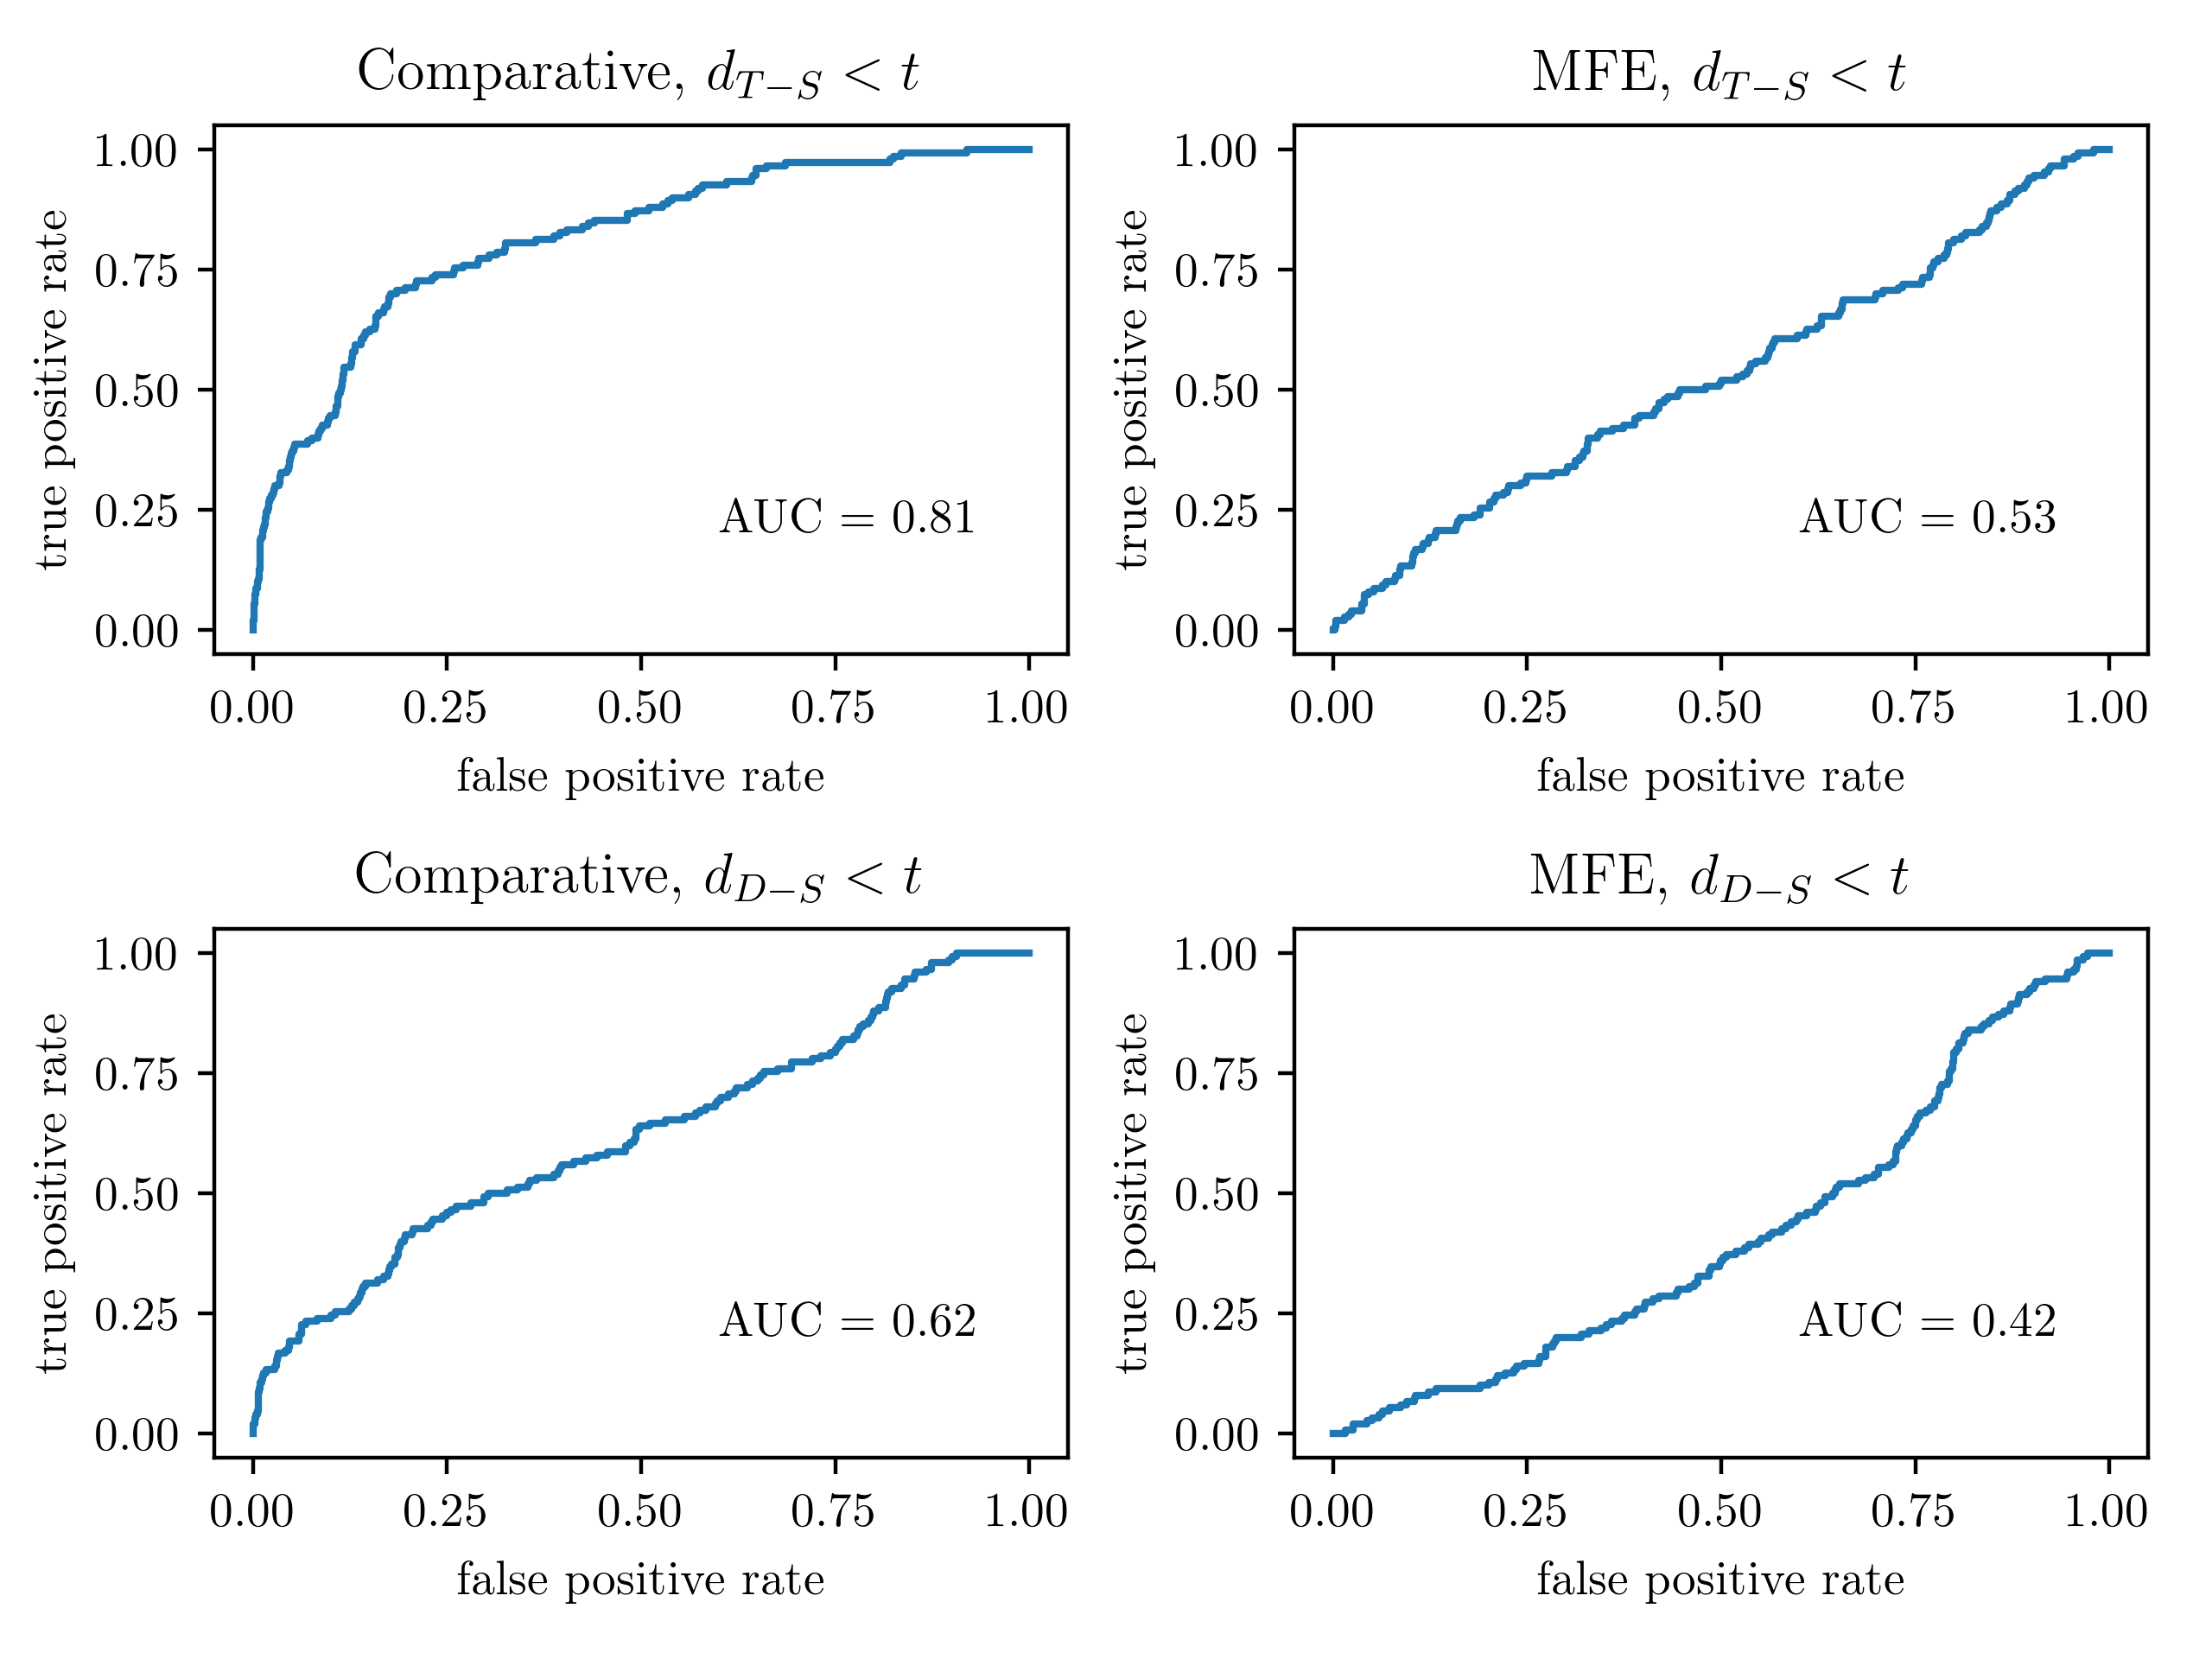
\includegraphics[width=0.7\textwidth]{bound_unbound.png}
\vglue 0.5cm

\caption{{\bf Bound or Unbound?} ROC performance of classifiers based on thresholding T-S
and D-S ambiguity indexes. Small values are taken as evidence for molecules that are active as
single entities (unbound), as opposed to parts of ribonucleoproteins (bound). Classifiers in the
left two panels use comparative secondary structures to compute ambiguity indexes; those on the
right use (approximate) minimum free energies. In each of the four experiments, a conditional
p-value was also calculated, based only on the signs of the indexes and the null hypothesis that
positive indexes are distributed randomly among molecules of all types as opposed to the alternative
that positive indexes are more typically found among families of bound RNA. Under the null hypothesis,
the test statistic is hypergeometric---see Eq \ref{eqn:null}. {\em Upper Left:} $p= 1.2 \times 10^{-34} $; {\em Lower Left:} $p=7.3 \times 10^{-8}$; {\em Upper Right:} $p=0.02$;  {\em Lower Right:} $p=0.92$. In considering these extreme p-values, it is perhaps worth re-emphasizing the points made about the interpretation of p-values in the paragraph following Eq \ref{eqn:null}.}  
\label{fig:UnboundVSBound}
\end{figure}


As mentioned earlier, we can also associate a traditional p-value to the problem of separating unbound from bound molecules, based on the T-S ambiguity indexes. We consider only the signs (positive or negative) of these indexes, and then test whether there are fewer than expected positive indexes among the unbound, as opposed to the bound, population. This amounts to computing $\mathbb{P}\{N\leq n_1\}$ from the hypergeometric distribution---Eq (\ref{eqn:null}). The relevant statistics can be found in Table \ref{table:NumberPositive}, 
under the column labels {\bf \#mol's} and $\bm \#d_\text{\bf T-S}>0$. Specifically, 
$M_1=116+34=150$ (number of unbound molecules),
$M_2=404+346+407+279+59=1495$ (number of bound molecules), $n_1=50+8=58$ (number of positive T-S indexes among unbound molecules) and $n_2=368+269+379+210+53=1279$.
The resulting p-value, $1.2\cdot 10^{-34}$, is essentially zero, meaning that the positive T-S indexes are not distributed proportional to the sizes of the unbound and bound populations, which is by now obvious, in any case. To repeat our caution, small p-values conflate sample size with effect size, and for that reason we have chosen additional ways, using permutations as well as classifications, to look at the data.

\vglue .1cm
\begin{table}[h!]
\begin{center}
\begin{tabular}{ l || r | r | r | r | r}
\hglue 5mm 
{\bf family} & {\bf \#mol's} & {\bf\#}$\bm{d_\text{\bf T-S}\!>\!0}$ &
{\bf\#}$\bm{d_\text{\bf D-S}\!>\!0}$ & {\bf\#}$\bm{d_\text{\bf \~T-\~S}\!>\!0}$ & {\bf\#}$\bm{d_\text{\bf \~D-\~S}\!>\!0}$ \\ \hline \hline
 Group I Introns & 116 & 50 & 100 & 94 & 114 \\  \hline
 Group II Introns & 34 & 8 & 21 & 27 & 33 \\  \hline
 tmRNA & 404 & 368 & 396 & 358 & 396 \\  \hline
 SRP RNA & 346 & 269 & 314 & 264 & 302 \\  \hline
 RNase P & 407 & 379 & 393 & 377 & 404 \\  \hline
 16s rRNA & 279 & 210 & 251 & 254 & 278 \\  \hline
 23s rRNA & 59 & 53 & 56 & 54 & 58 \\  \hline

\end{tabular}
\vglue .5cm
\caption{\footnotesize {\bf Numbers of Positive Ambiguity Indexes, by family.} 
{\bf \#mol's}: number of molecules; {\bf\#}$\bm{d_\text{\bf T-S}>0}$ and 
 {\bf\#}$\bm{d_\text{\bf D-S}>0}$: numbers of positive T-S and D-S ambiguity indexes, secondary structures computed by {\em comparative analysis}; 
 {\bf\#}$\bm{d_\text{\bf \~T-\~S}>0}$ and {\bf\#}$\bm{d_\text{\bf \~D-\~S}>0}$: numbers of positive T-S and D-S ambiguity indexes, secondary structures computed by {\em minimum free energy}.
} 
\label{table:NumberPositive}
\end{center}
\end{table}

The comparative secondary structure of an RNA molecule, when combined with its primary structure, can be used to construct a measure---the T-S ambiguity index---which distinguishes unbound from bound molecules with good accuracy. Can the same can be said for the D-S index?
Yes, albeit with lower accuracy. To demonstrate, we followed the identical procedure, except that we assigned the index $d_\text{D-S}(p,s)$ rather than $d_\text{T-S}(p,s)$ to each molecule.  The ROC curve (with area 0.62) is shown in the lower-left panel of Figure \ref{fig:UnboundVSBound}. The hypergeometric test, based on the thresholded (signed) values of  $d_\text{D-S}$ (positive counts, for each RNA family, can be found in Table \ref{table:NumberPositive}) has p-value $7.3\cdot 10^{-8}$. Finally, the right-hand panels in Figure \ref{fig:UnboundVSBound} mirror the left-hand panels, except that all secondary structures were computed by (approximately) maximizing free energy rather than comparative analysis. The classification results are substantially less convincing and the p-values substantially higher.  

\subsubsection*{Comparative Analysis versus Minimum Free Energy}
As we have just seen, ambiguity indexes based on MFE secondary structures, as opposed to  comparative secondary structures, do not make the same stark 
distinction between single and bound RNA molecules. 
To explore this a little further, we can turn the analyses of the previous paragraphs around
and ask to what extent knowledge of the group of a molecule (unbound or bound) and its ambiguity index (e.g. the T-S ambiguity index) is sufficient to predict the source of the secondary structure---comparative or free energy? 

Interestingly, there is a sharp difference in predicting the source of secondary structure in unbound molecules as opposed to bound molecules. Consider the top two ROC curves in Figure
\ref{fig:CompVSMFE}. In each of the two experiments a classifier was constructed by thresholding the T-S ambiguity index, declaring the secondary structure to be 
`comparative' when $d_\text{T-S}(p,s)<t$ and `MFE' otherwise, since, as we have seen, smaller values of the ambiguity indexes are generally associated with the comparative secondary structure. The ROC curves are then swept out by varying $t$. The difference between the two panels is in the population used for the classification experiments---unbound molecules in the upper-left and bound molecules in the upper-right. In unbound molecules, small values of the T-S ambiguity index are a good indication that a secondary structure was derived from comparative rather than free-energy analysis, but not in bound molecules. The corresponding hypothesis tests seek evidence against the null hypotheses that in a given group (unbound or bound) the set of positive T-S ambiguity indexes ($d_\text{T-S}(p,s)>0$) are equally distributed between the comparative and free-energy derived indexes, and in favor of the alternatives that the T-S ambiguity indexes are less typically positive for the comparative secondary structures. The necessary data can be found in Table \ref{table:NumberPositive}. The results are consistent with the classification experiments: the hypergeometric p-value is 
is $5.4\cdot 10^{-14}$ for the unbound population and $0.07$ for the bound population.

The same experiments, with the same conclusions, were also performed using the D-S ambiguity index, as shown in the bottom two panels of Figure \ref{fig:CompVSMFE}, for which the corresponding hypergeometric p-values are $3.8\cdot 10^{-7}$ (unbound population) and $0.01$ (bound population). 


\begin{figure}[h!]
\centering
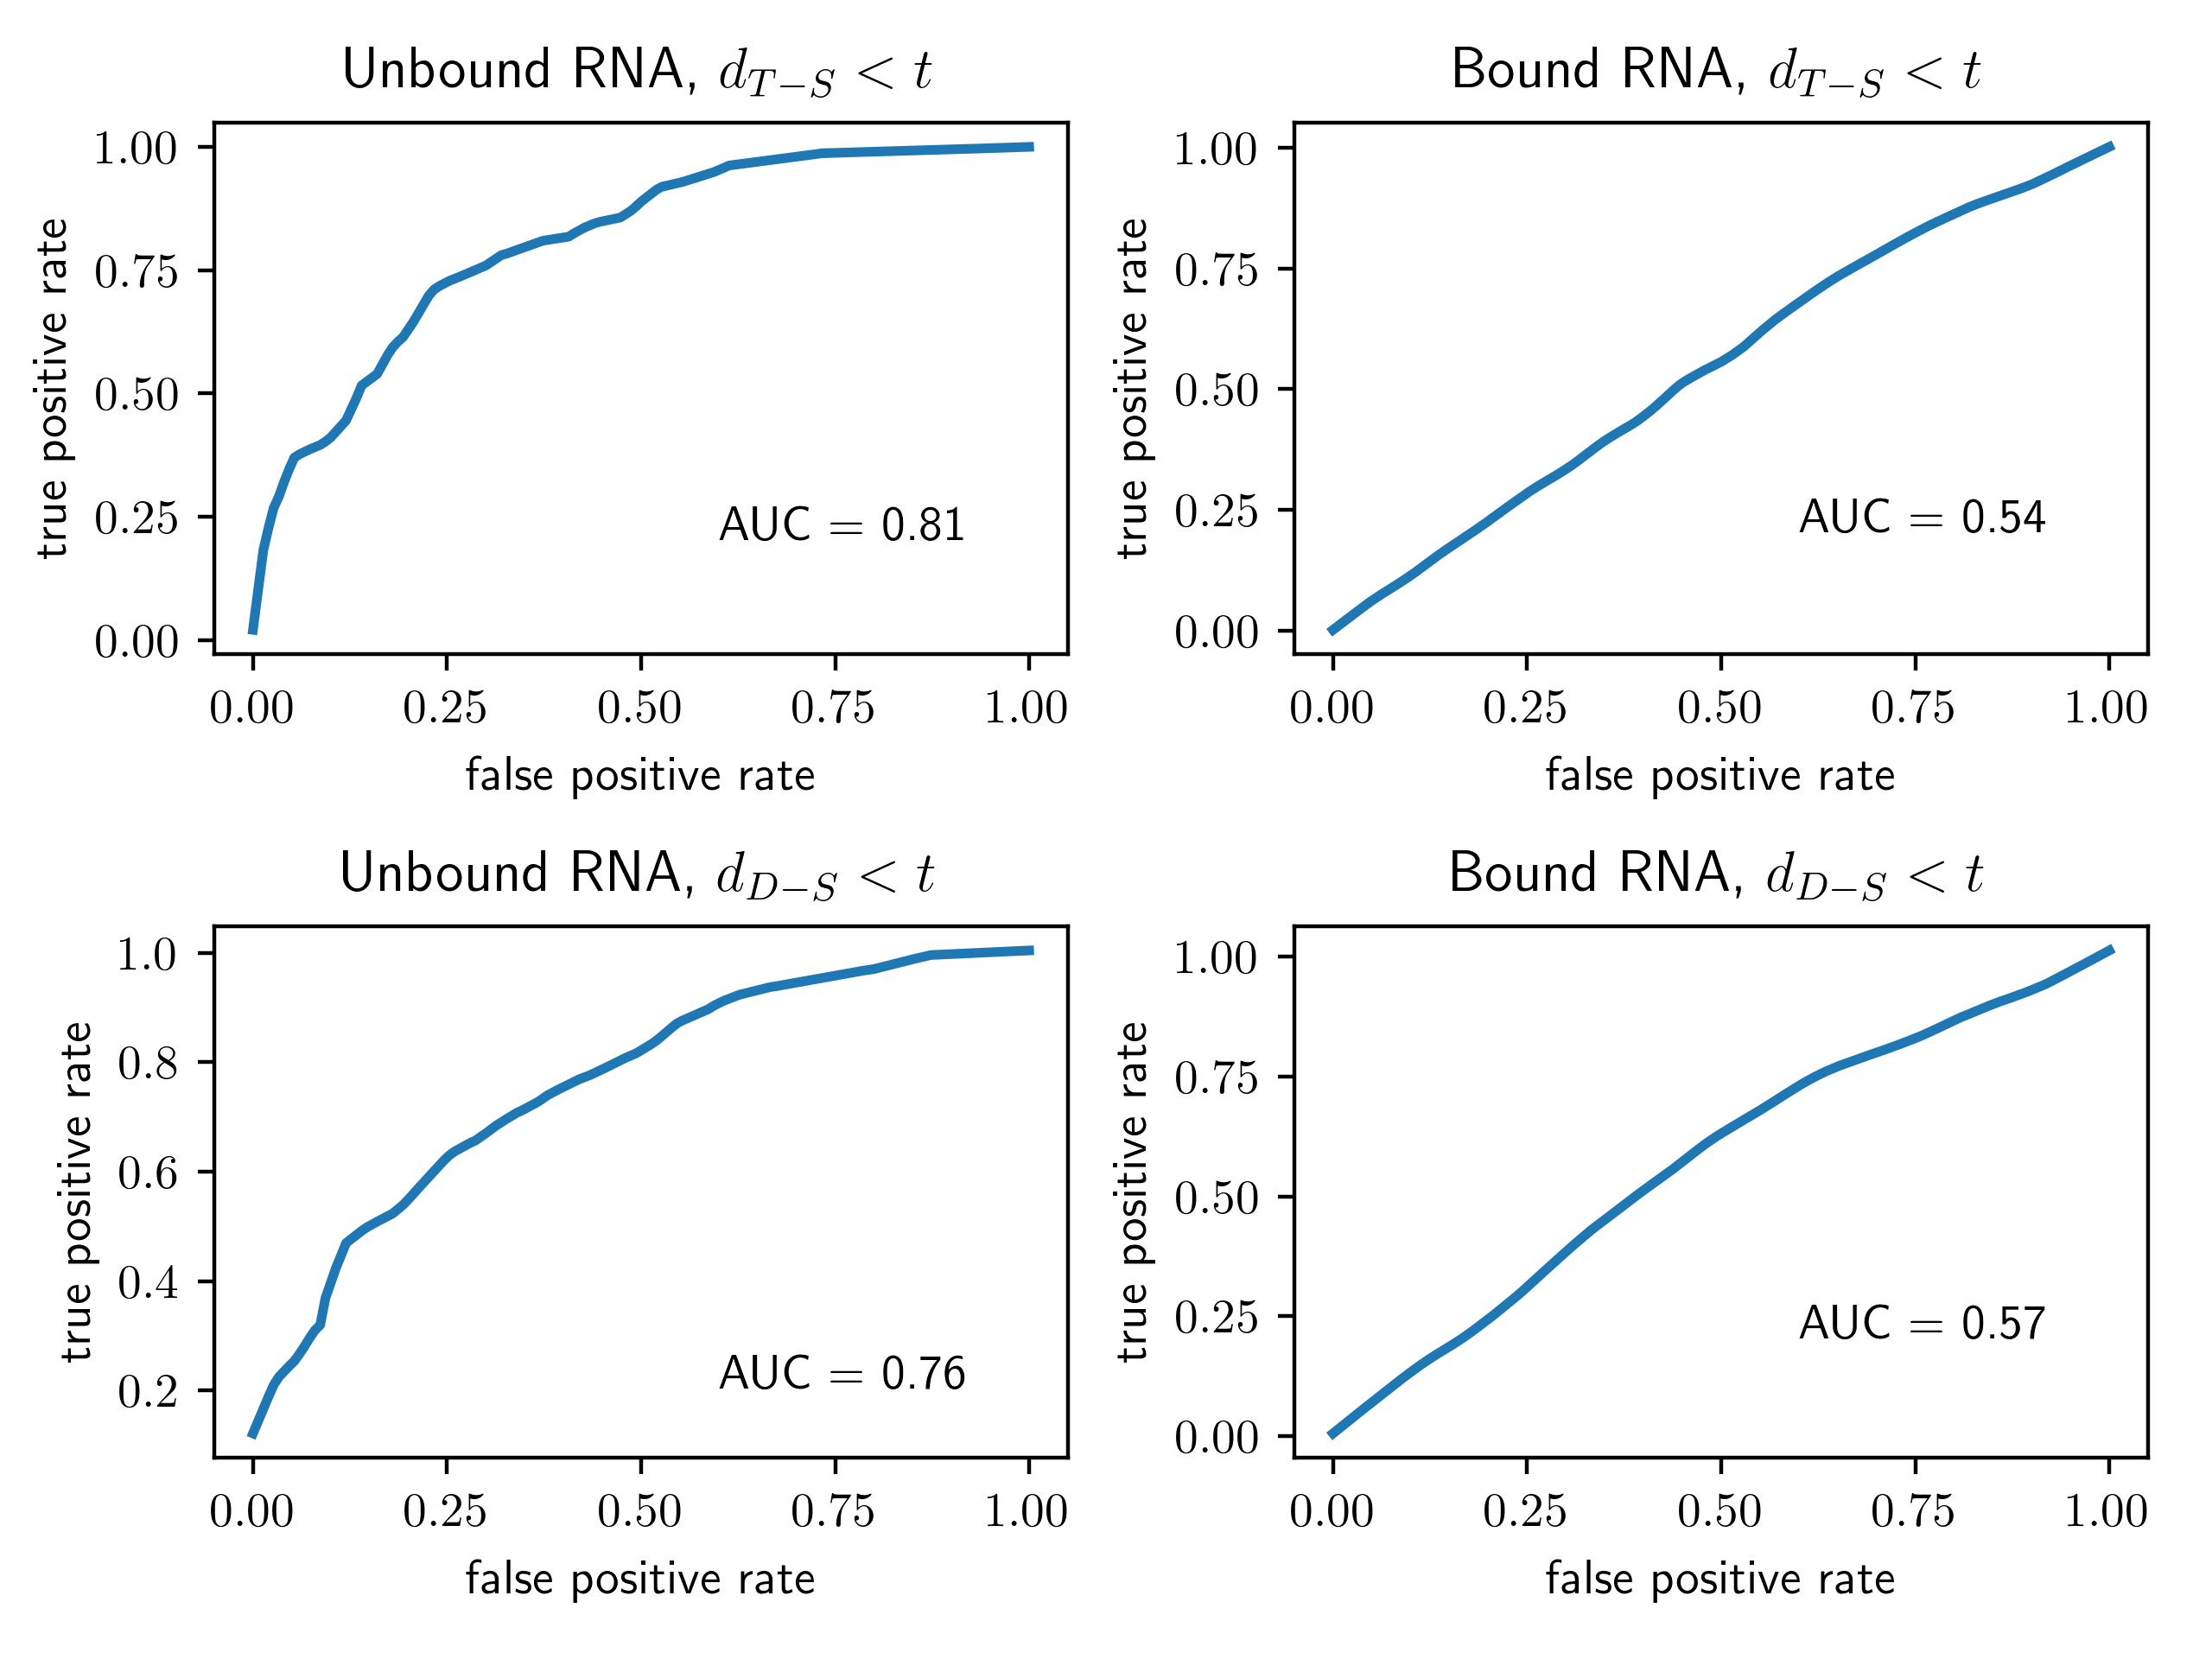
\includegraphics[width=0.7\textwidth]{comparative_mfe.png}
\vglue 0.5cm

\caption{{\bf Comparative or MFE?} As in Figure \ref{fig:UnboundVSBound}, each panel
depicts the ROC performance of a classifier based on thresholding the T-S (top two panels) or
D-S (bottom two panels) ambiguity indexes. Here, small values are taken as evidence for
comparative as opposed to MFE secondary structure. Either index, T-S or D-S, can be used to
construct a good classifier of the origin of a secondary structure for the unbound molecules in
our data set (left two panels) but not for the bound molecules (right two panels). Conditional
p-values were also calculated, using the hypergeometric distribution and based only on the signs
of the indexes. In each case and the null hypothesis is that comparative secondary structures are as
likely to lead to positive ambiguity indexes as are MFE structures, whereas the alternative is
that positive ambiguity indexes are more typical when derived from MFE structures:
{\em Upper Left:} $p= 5.4 \times 10^{-14} $; {\em Upper Right:} $p=0.07$; {\em Lower Left:} $p=3.8 \times 10^{-7}$;  {\em Lower Right:} $p=0.01$.}
\label{fig:CompVSMFE}
\end{figure}


\section*{Discussion}

%From the above results, we can see that we verified a lot of the suspicions we had in the discussions of the exploratory analysis results. We demonstrated that we can indeed statistically seperate \textit{single-entity RNAs} from \textit{protein-RNA complexes}, using the ``ambiguity index". We can also statistically seperate the \textit{comparative analysis} structures from the \textit{minimum free energy} structures for \textit{single-entity RNAs}, using the ``ambiguity index", but we can't achieve this when we look at \textit{protein-RNA complexes}.
%
%These results suggest a potentially significant difference between the structure formation mechanisms on \textit{single-entity RNAs} and \textit{protein-RNA complexes}, and a qualitative difference between the \textit{comparative analysis} methods and the \textit{minimum free energy} methods when applied to \textit{single-entity RNAs}.
%
%Possible that MFE methods are way off, or that much better answers come from equilibrium samples or even centroids...
%
%in vivo structure is a compromise between stability and accessibility. 
%
%Our reasoning is mechanistic. 
%
%Given a favorable tertiary structure, it is likely that many nucleotide substitutions 
%This reasoning, mechanistic, 
%
%``Under Construction''!!!
%
%******
%The goal of this paper is to present statistical evidence that supports a a kinetic, but not necessarily equilibrium, viewpoint of RNA structure. verify our basic intuition, by looking at the differences in terms of local ambiguity between locations that participate in the secondary structure and the locations that don't, and to establish an intra-molecular statistical relationship between secondary and primary structures. This is achieved by some exploratory analysis as well as two sets of exact and highly significant hypothesis tests, which unveil fascinating results on the local ambiguities in different regions of the RNA molecules, the possible mechanistic differences in the structure formation of single-entity RNAs and protein-RNA complexes, as well as the subtle differences between the comparative analysis approach and the minimum free energy approach for RNA secondary structure prediction.
%**********
%
%Mention another possible statistical signature: stems that are phylogenetically older tend to be formed earlier in the folding process
%
%First, from the experiments and the results in this paper, ``local ambiguity" clearly emerges as a useful concept in the statistical analysis of RNA primary and secondary structure data and the folding process of RNA molecules.
%
%Based on ``local ambiguity", an ``ambiguity index'', one for each pair of molecule and presumed secondary structure, measures the prevalence of false matches and hence the tendency to form metastable structures  incompatible with native structures. The ambiguity index statistically separates an ensemble of RNA molecules that operate as single entities (Group I and II Introns) from an ensemble that operates as protein-RNA complexes (SRP and tmRNAs), and ensembles of secondary structures determined by comparative analysis from ones based on thermal equilibrium. We find lower average ambiguity in single-entity RNA's than protein-RNA complexes, and, among single-entity RNA's, lower ambiguity with comparative analyses than equilibrium analyses. These results demonstrate possible mechanistic differences in the structure formation of single-entity RNAs, where kinetics play a more important role, and protein-RNA complexes, where the protein-RNA interactions have significant impacts on the folding process, and a qualitative difference between the comparative analysis approach and the minimum free energy approach in the case where kinetics are important (in this paper, for single-entity RNAs).
%
%
%
%These empirical evidence points to the importance of carefully considering the impacts of kinetics and protein-RNA interactions on the folding process of non-coding RNA molecules, and argues against the naive application of thermal equilibrium based approaches for RNA secondary structure prediction.

\section*{Materials and Methods}
\subsection*{Datasets}

In this paper, we obtained comparative analysis secondary structures data for seven different families of RNA molecules from the RNA STRAND database\cite{Andronescu2008-rj}, a curated collection of RNA secondary structures. These families include: Group I Introns and Group II Introns\cite{Cannone2002-tp}, tmRNAs and SRP RNAs\cite{Andersen2006-uh}, the Ribonuclease P RNAs\cite{Brown1999-co}, and 16s rRNAs and 23s rRNAs\cite{Cannone2002-tp}. Table \ref{table:lengths} contains information about the numbers and lengths (measured in nucleotides) of the RNA molecules in each of the seven groups studied. Note that we excluded families like tRNAs, 5s rRNAs and hammerhead ribozymes since most of the molecules in these families are too short to be interesting for our purpose. Also, since we are focusing on comparative analysis secondary structures, we excluded any secondary structures derived using x-ray crystallography or NMR.

\vglue .1cm
\begin{table}[h!]
\begin{center}
\begin{tabular}{ l || r | r | r| r}
\hglue 5mm {\bf family} & {\bf number} & {\bf min length} & {\bf max length} & {\bf median} \\ \hline \hline
 Group I Introns & 116 & 210 & 2630 & 451 \\ \hline
 Group II Introns & 34 & 619 & 2729 & 990 \\ \hline
 tmRNA & 404 & 102 & 437 & 363 \\ \hline
 SRP RNA & 346 & 66 & 533 & 274 \\ \hline
 RNase P & 407 & 189 & 486 & 330 \\ \hline
 16s rRNA & 279 & 612 & 2394 & 1512 \\ \hline
 23s rRNA & 59 & 953 & 4381 & 2913 \\ \hline

\end{tabular}
\vglue .5cm
\caption{\footnotesize {\bf Data Summary.} The seven families of RNA used in the experiments. Table includes the number of molecules in each family, as well as basic statistics about the numbers of nucleotides in the primary sequence of each of the molecules. Data was downloaded from the \href{http://www.rnasoft.ca/strand/}{RNA STRAND database}.}
\label{table:lengths}
\end{center}
\end{table}


\subsection*{Minimum Free Energy Methods}

Exact dynamic programming algorithms based on carefully measured thermodynamic parameters are still the prevalent methods for RNA secondary structures prediction. There exist a large number of software packages for the energy minization \cite{Lorenz2011-eb, Markham2008-ku, Reuter2010-bw, Zadeh2011-eu, Hamada2009-yf, Ding2003-sv, Reeder2009-xl}. In this paper, we used the \href{https://www.tbi.univie.ac.at/RNA/}{ViennaRNA package} \cite{Lorenz2011-eb} to obtain the MFE secondary structures for our statistical analysis.

\subsection*{Reproducing the Results}
The results presented in this paper can be easily reproduced. Follow the intrustions on \url{https://github.com/StannisZhou/rna_statistics}. Here we make a few comments regarding some implementation details.
\begin{itemize}
	\item In the process of obtaining the data, we used the \textit{bpseq} format, and excluded structures derived from x-ray crystallography or NMR structures, as well as structures for duplicate sequences. Concretely, this means picking a particular type, and select \textit{No} for \textit{Validated by NMR or X-Ray} and \textit{Non-redundant sequences only} for \textit{Duplicates} on the \href{http://www.rnasoft.ca/strand/search.php}{search page} of the RNA STRAND database. A copy of the data we used is included in the \href{https://github.com/StannisZhou/rna_statistics/tree/master/data}{GitHub repository}, but the readers should feel free to try out the analysis on other data.
	\item When processing the data, we ignored molecules for which we have nucleotides other than \textit{A, G, C, U}, and molecules for which we don't have any base pairs.
	\item When comparing the local ambiguities in different regions of the RNA molecules, we ignored molecules for which we have empty regions (i.e. at least one of \textit{single, double} and \textit{transitional} is empty), as well as molecules where all local ambiguities in \textit{single} or \textit{double} are 0.
	\item For shuffling the molecules, we used an efficient and flexible implementation of the Euler algorithm\cite{Kandel1996-kz, Fitch1983-ec, Altschul1985-nq}, called uShuffle \cite{Jiang2008-yj}, which is conveniently available as a \href{https://github.com/guma44/ushuffle}{python package}.
\end{itemize}

\section*{Acknowledgments}

\section*{Appendix}

\nolinenumbers

\bibliography{reference.bib}

\end{document}
